%FOR PDFLATEX USE ONLY
\documentclass[a4paper,12pt]{article}

\usepackage{amssymb,amsmath} %math symbols

\usepackage[margin=2cm]{geometry} %paper geometry

\usepackage[utf8]{inputenc} %allows unicode (including russian) source file
\usepackage[russian]{babel} %docment in russian-style
\usepackage[utf8]{inputenc}
\usepackage[unicode]{hyperref} %links inside of the text
\usepackage[pdftex]{graphicx} %includegraphics pictures
\usepackage{cmlgc} %bold text

\usepackage{array} %arrays

\usepackage{wrapfig}
\usepackage{array}
\usepackage{lipsum}
\usepackage{esvect}
\usepackage{hyperref}
\usepackage{xcolor}
\definecolor{linkcolor}{HTML}{799B03} % цвет ссылок
\definecolor{urlcolor}{HTML}{799B03} % цвет гиперссылок
 
\hypersetup{pdfstartview=FitH,  linkcolor=linkcolor,urlcolor=urlcolor, colorlinks=true}
 
\usepackage{subfig}
\usepackage{calc}
\usepackage{pgfplots,tikz,circuitikz}
\usepackage{pgfplotstable}
\usepackage{tkz-euclide}

\usepackage{centernot}
\usepackage{cancel}

\documentclass{article}
\usepackage{amsmath}
\usepackage{mathtext}
\usepackage[T1,T2a]{fontenc}
\usepackage[utf8]{inputenc}
\usepackage[english, bulgarian, russian]{babel}
\usepackage{tikz}
\usepackage{pgfplots}
\usepackage[export]{adjustbox}
\usepackage[left=2cm,right=2cm,
    top=2cm,bottom=2cm,bindingoffset=0cm]{geometry}

\begin{document}



\maketitle
\begin{center}
\LARGE{МОЛЕКУЛЯРНАЯ ДИНАМИКА}\\
    \Large{Задание 2}\\
    Стрижак Даниил
\end{center}
\tableofcontents
\newpage

\section{Аннотация}
 Данная работа сделана с помощью lammps. Из-за того, что на то, чтобы разобраться с симулятором, потребовалось много времени, графики будут не лучшего качества. \\
 В каждом пункте (кроме 5) расссчет производится с шагом $t = 0.005$ в количестве 10000 шагов. 
 
 
\section{Радиальная функция распределения}

Для 2 параметров плотности и температуры входного файла построим радиальные функции расперделения. 

\begin{minipage}{0.47\textwidth}
    $$ \rho = 0.7$$
    $$T = 1.0 $$
    \begin{center}
        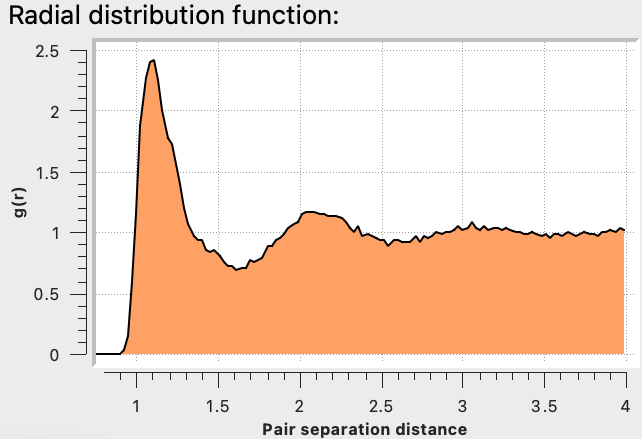
\includegraphics[width=\linewidth]{1.png}\\
        Плотная жидкость
    \end{center}
   
\end{minipage}
\begin{minipage}{0.47\textwidth}
    $$ \rho = 0.01$$
    $$T = 1.0 $$
    \begin{center}
        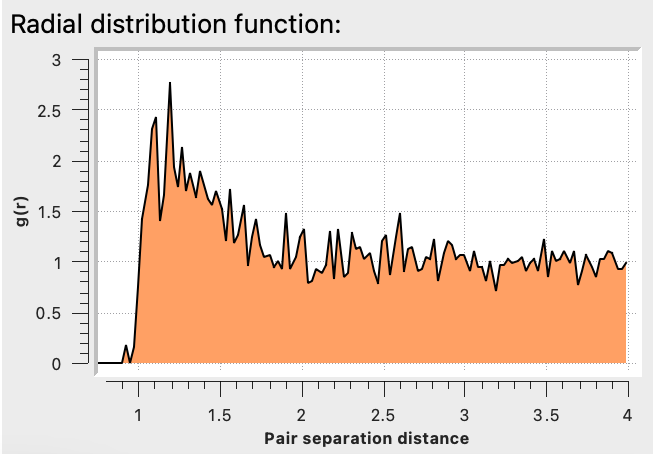
\includegraphics[width=\linewidth]{2.png}\\
        Газ
    \end{center}
\end{minipage}

\
\newline			

В сравнении с экспериментальной работой Yarnell et al. можно сделать вывод, что данные сходятся. Для жидкостной зависимости все экстремальные характеристики совпадают. В обоих случаях RDF стремится к 1 при больших r. 

\section{Автокоррелятор скорости}

Аналогично предыдущему пункту построим автокорреляционные функции для жидкости и газа при тех же начальных параметрах, видно, что характер автокорреляционной функции проявляется, однако качество оставляет желать лучшего.  \\

\newline

\begin{minipage}{0.47\textwidth}
    \begin{center}
        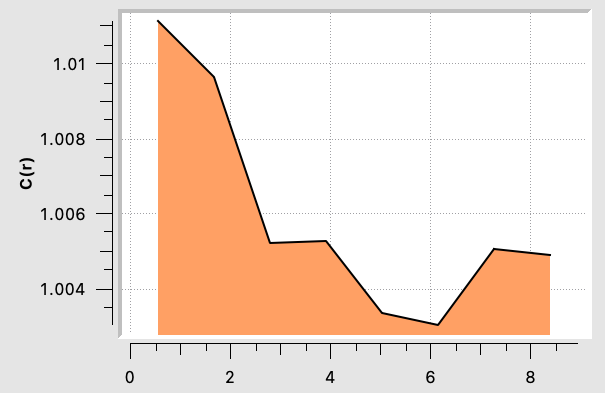
\includegraphics[width=\linewidth]{4.png}\\
        Плотная жидкость
    \end{center}
   
\end{minipage}
\begin{minipage}{0.47\textwidth}
    \begin{center}
        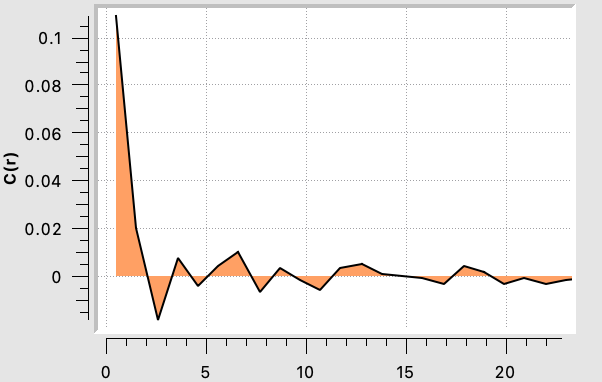
\includegraphics[width=\linewidth]{3.png}\\
        Газ
    \end{center}
\end{minipage}



\section{Коэффициент самодиффузии}

Рассчитаем коэффициент самодиффузии через формулы Эйнштейна-Смолуховского и Грина-Кубо для T = 1.0, 1.5, 2.0 и плотности 0.7. \\

\newline

\begin{minipage}{0.45\textwidth}
    \begin{center}
    \underline{Метод Эйнштейна-Смолуховского}
    $$D = \frac16\frac{\left\langle\mathbf r^2\right\rangle}t $$
    \begin{itemize}
    \item T = 1.0\\
    
    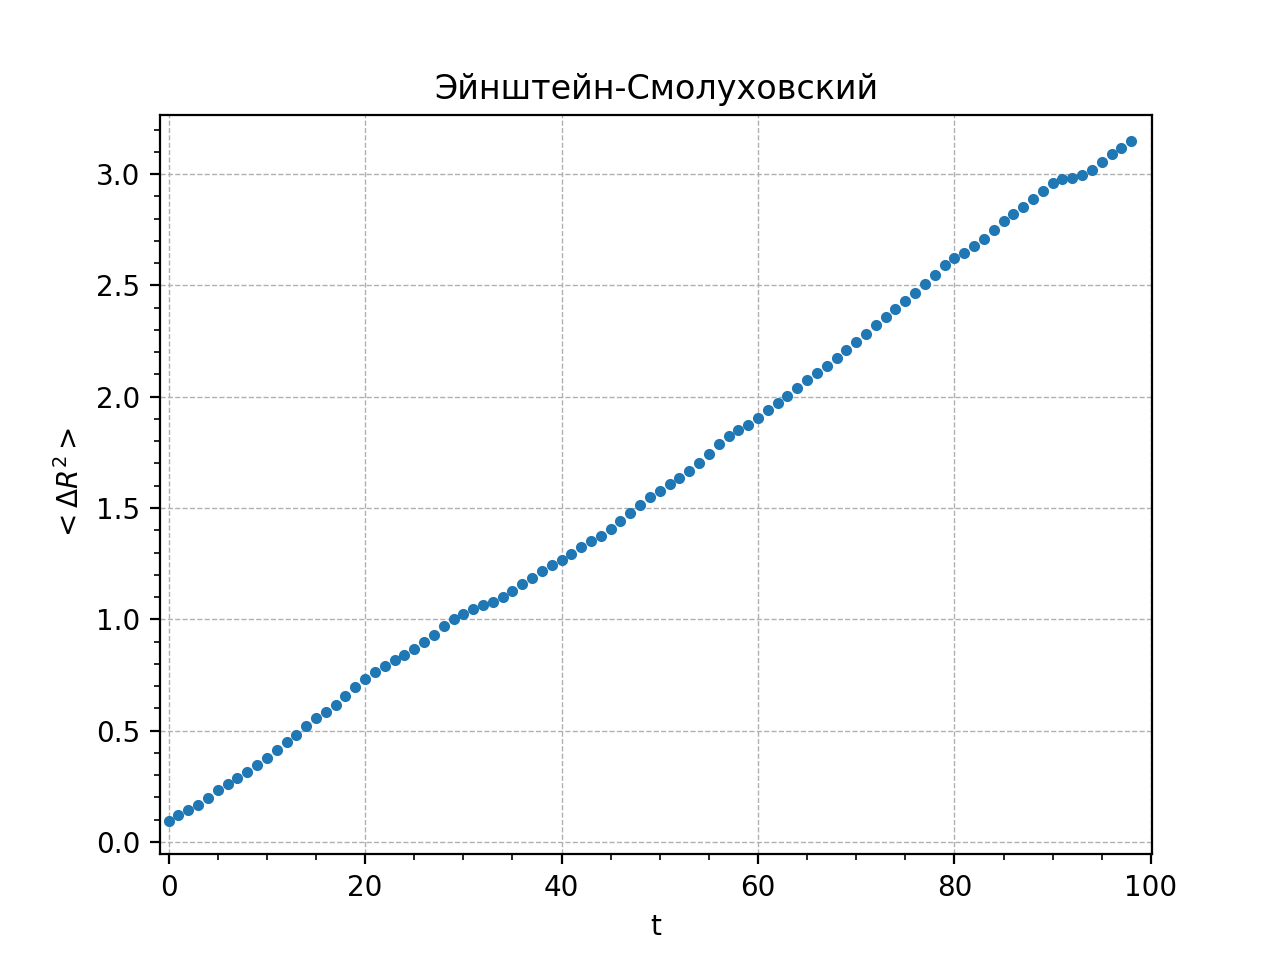
\includegraphics[width=\linewidth]{a.png}\\
    
    \item T = 1.5\\
    
    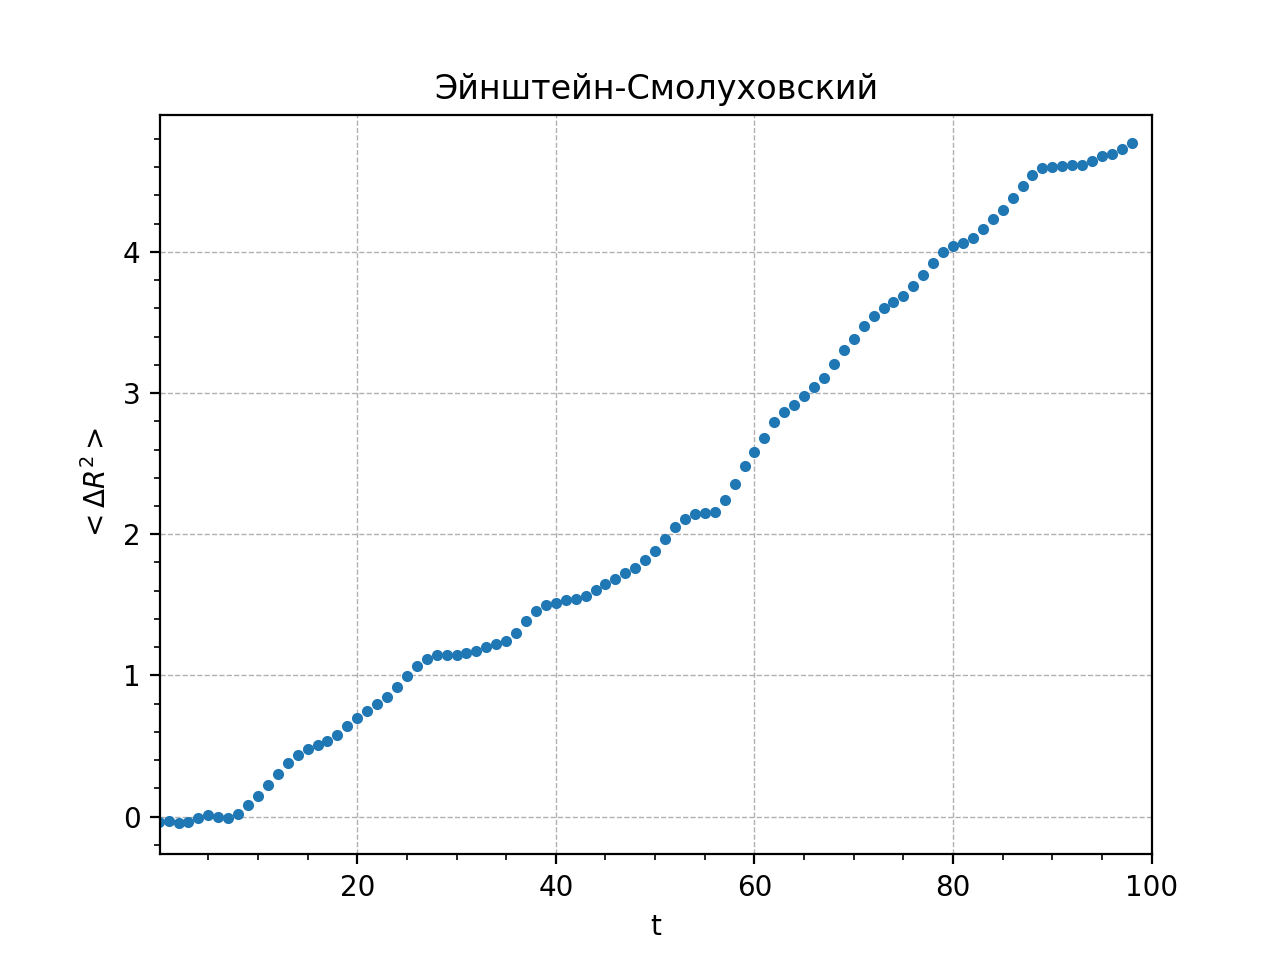
\includegraphics[width=\linewidth]{b.png}\\
    
    \item T = 2.0\\
    
    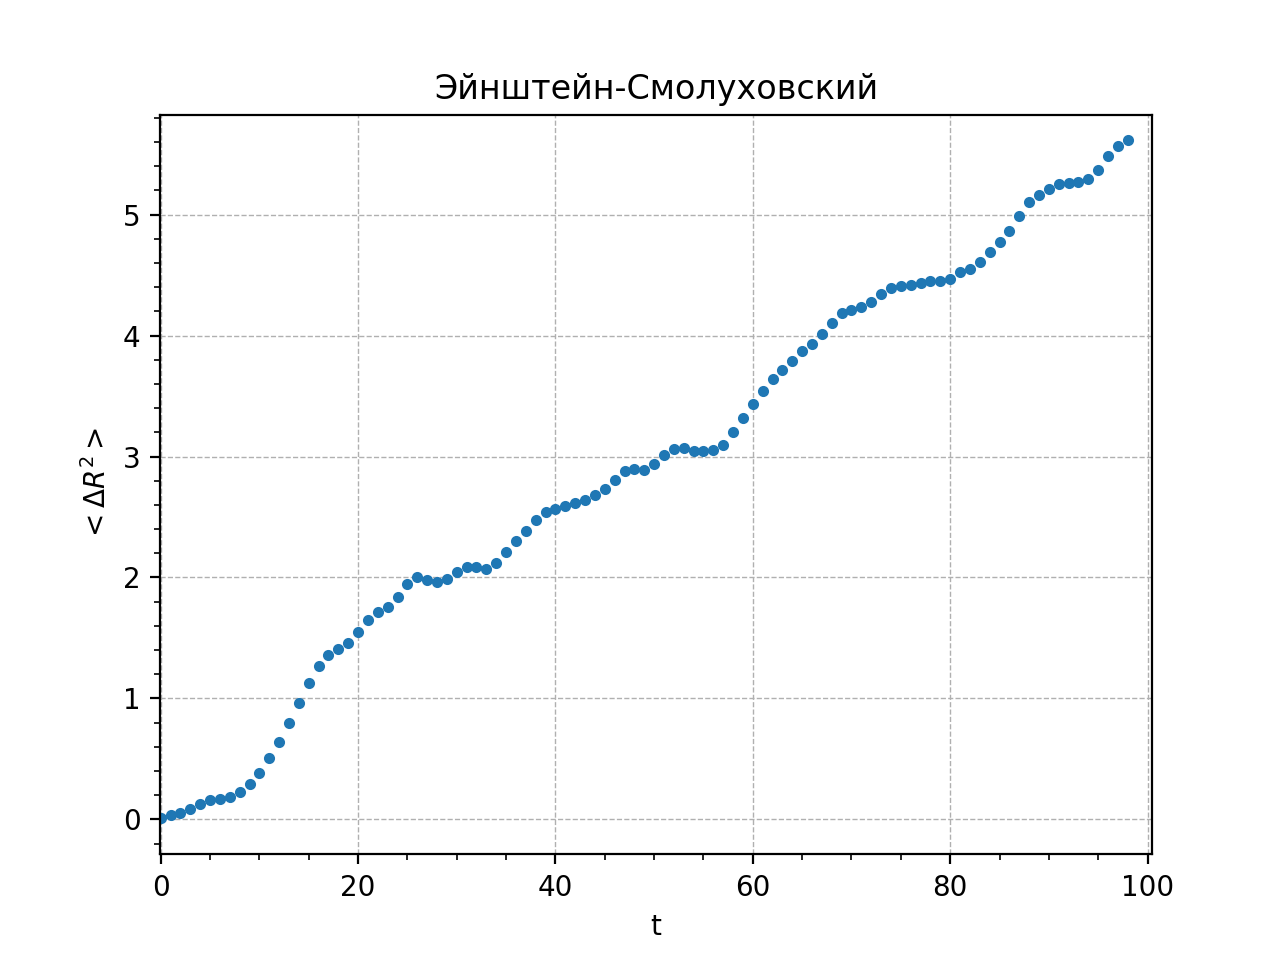
\includegraphics[width=\linewidth]{c.png}\\
    
    \end{itemize}
    \end{center}
\end{minipage}
\hfill\vline{\vrule width 1pt}\hfill
\begin{minipage}{0.45\textwidth}
    \begin{center}
    \underline{Метод Грина-Кубо}
    $$D=\frac{1}{3} \int_{0}^{\infty}\left\langle\mathbf{v}_{i}(t) \cdot \mathbf{v}_{i}(0)\right\rangle d t = \frac13S$$
    \begin{itemize}
    \item T = 1.0\\
    
    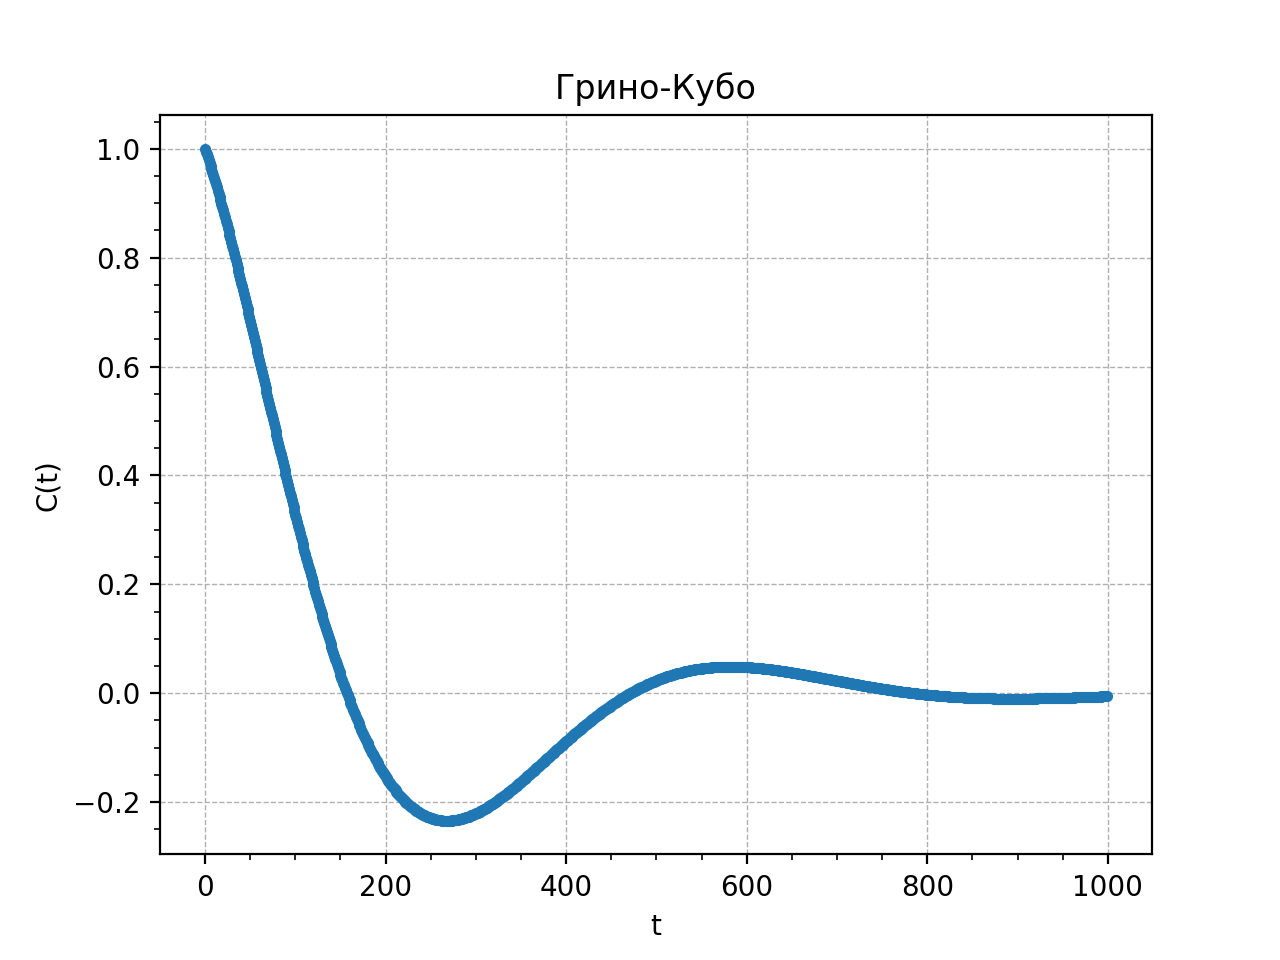
\includegraphics[width=\linewidth]{d.png}\\
    
    \item T = 1.5\\
    
    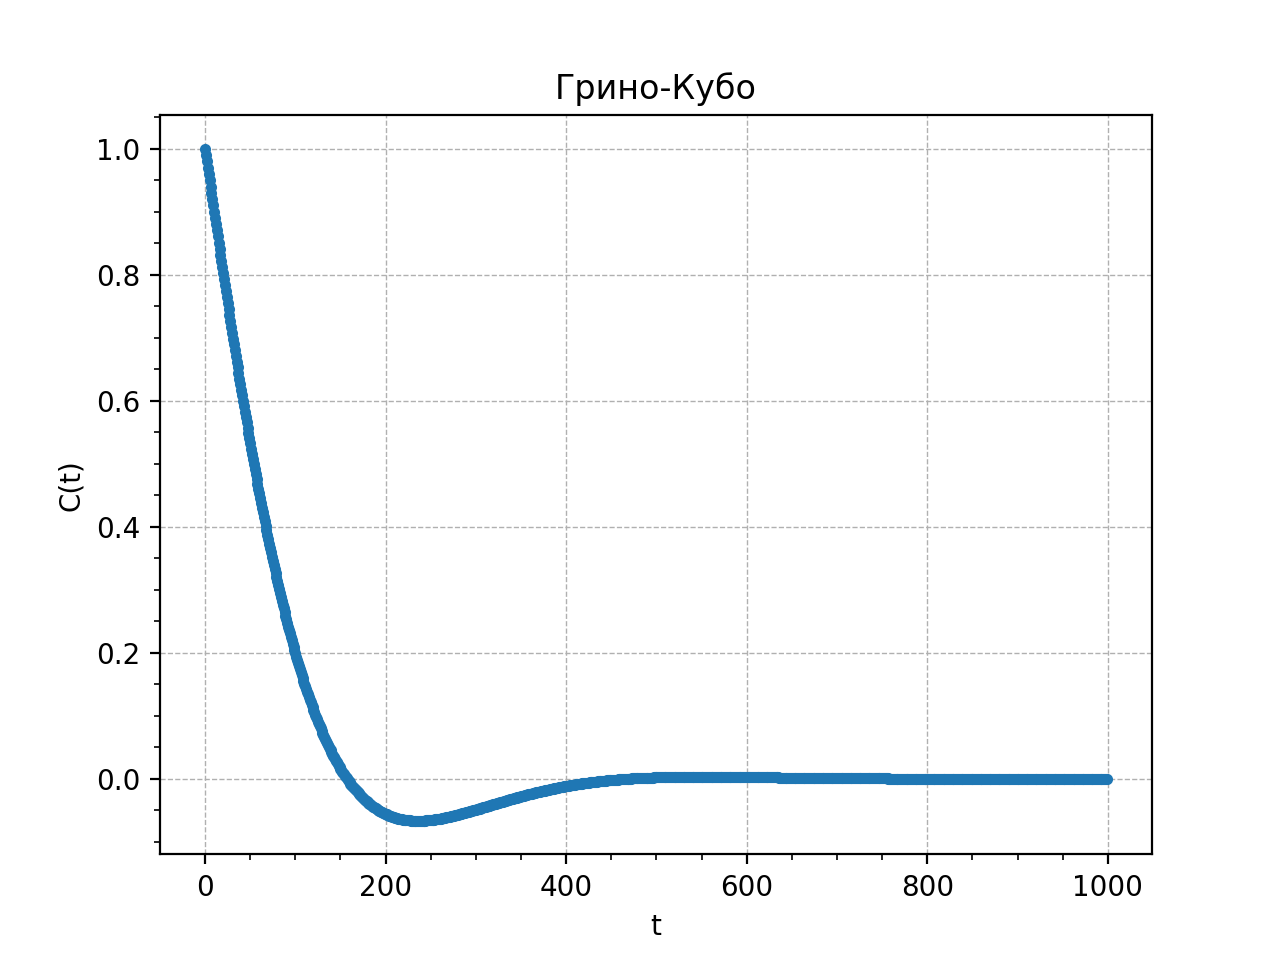
\includegraphics[width=\linewidth]{e.png}\\
    
    \item T = 2.0\\
    
    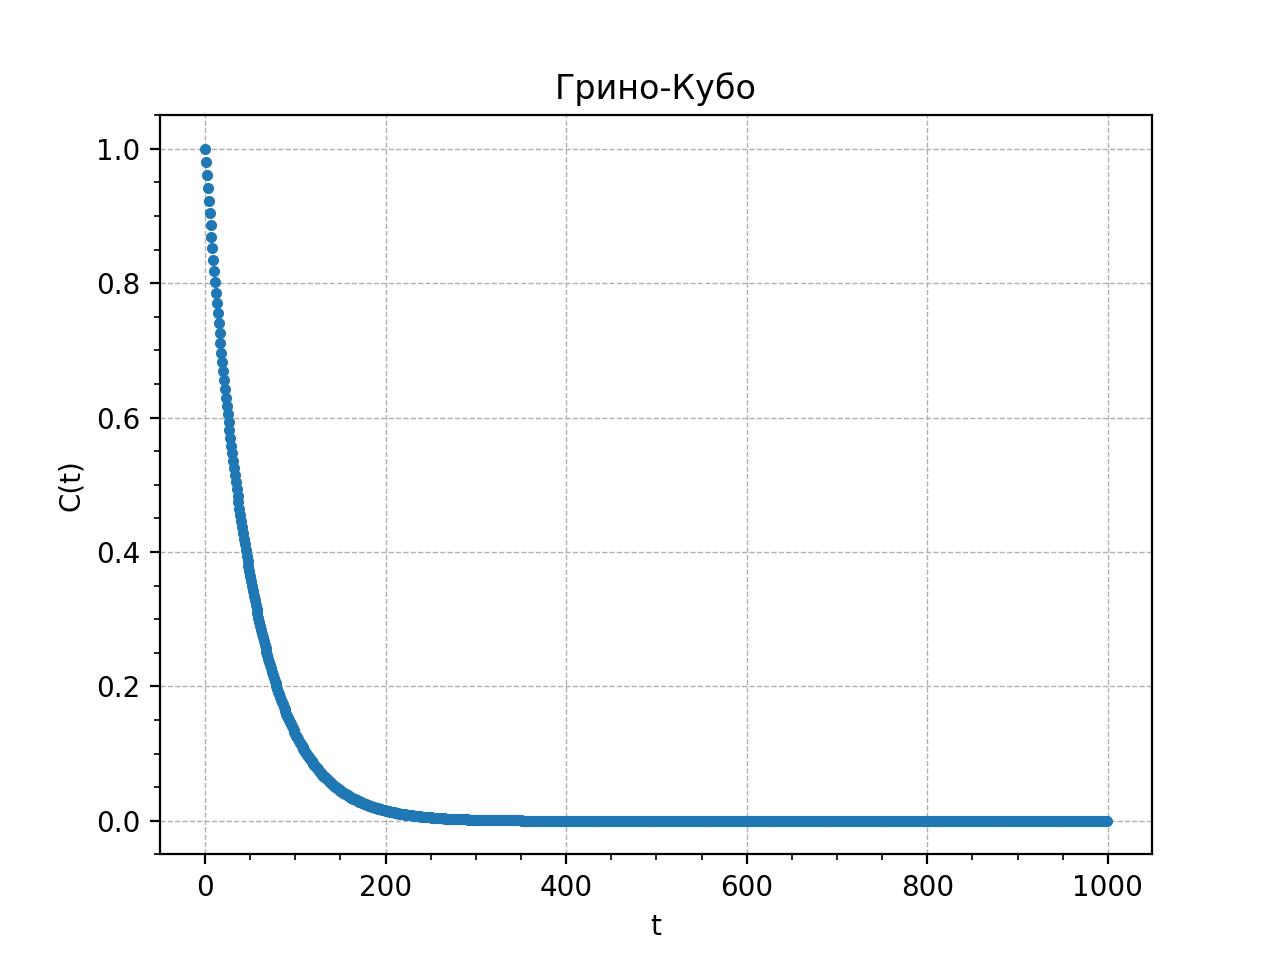
\includegraphics[width=\linewidth]{f.png}\\
    
    \end{itemize}
    \end{center}
\end{minipage}

\

\newline

Сведем полученные результаты в таблицу. Можно сделать вывод, что значения коэффициентов диффузии отличаются, но не более чем на 10\%. Значения, полученные методом Грина-Кубо получились немного заниженными. 

\begin{center}
\begin{tabular}{|c|c|c|c|}
\hline
T&Reference& E-S&G-K \\
\hline
1.0&0.105 &0.095&0.93	\\
\hline
1.5&0.156&0.149&0.141	\\
\hline
2.0&0.202&0.198&0.192	\\
\hline
\end{tabular}
\end{center}

\newpage

\section{Сравнение с невязками}

Рассчитаем невязки для двух разных времен рассчета t = 0.005 и t = 0.05 и отнормируем на линейный участок. Можно сделать вывод, что значения совпадают с референсной статьей. 

 $$\left\langle(R''-R')^2  \right\rangle = 12Dt$$
 $$D = 1.023 $$

 \begin{center}
   

    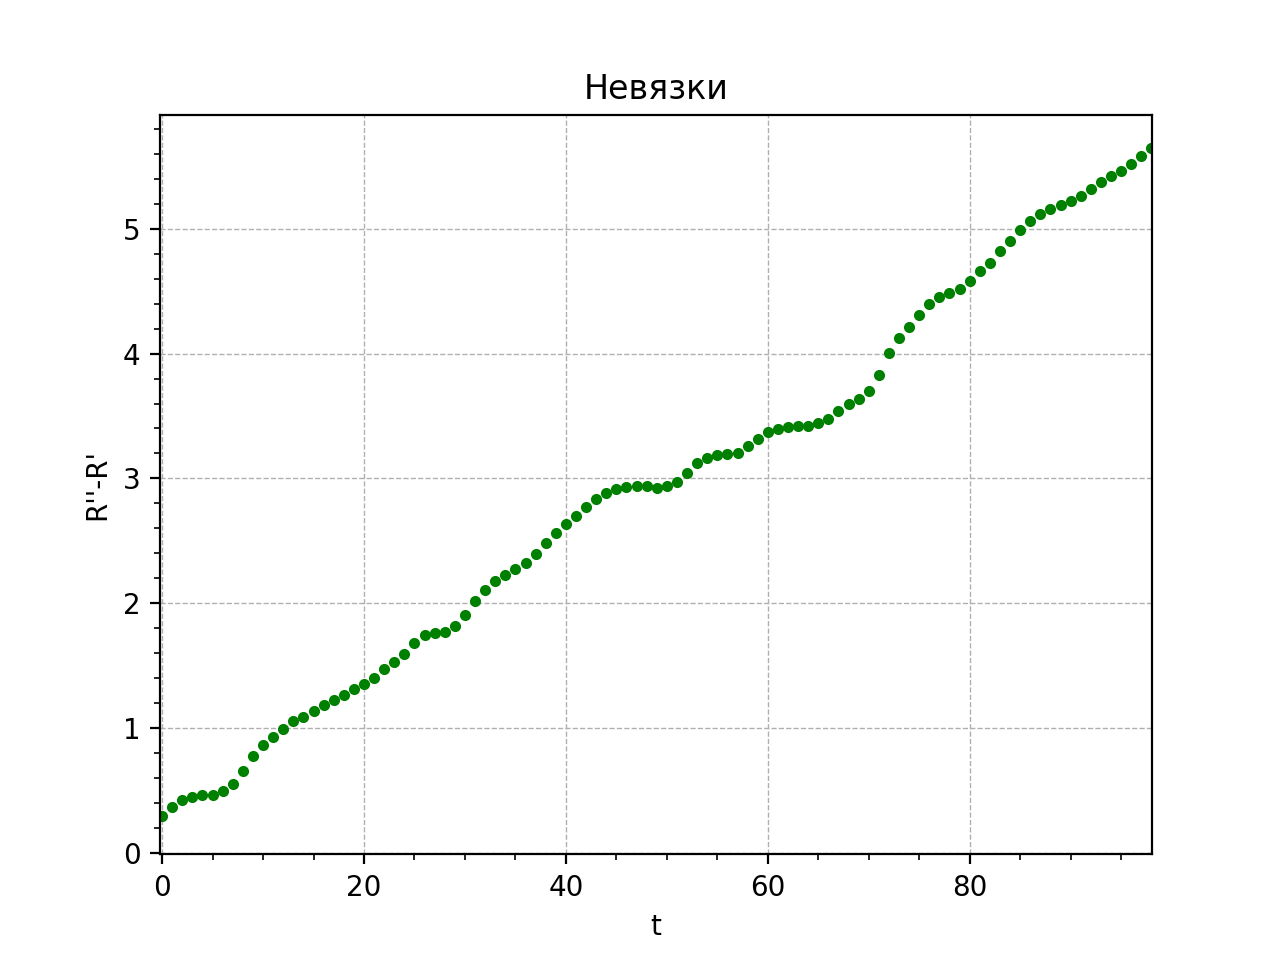
\includegraphics[width=\linewidth]{name.png}\\
    \end{center} 

\section{Влияние термостата}

Добавим условие термостата в lammps:\\ "fix ID group-ID nvt keyword\_value Tstart Tstop Tdamp".\\
Проверим коэффициенты диффузии с такой поправкой. \\

Из полученных результатов можно сделать вывод, что значения коэффициентов диффузии слабо отличаются от тех, что были получены ранее. ($D_{1.0} = 0.098\quad D_{2.0} = 0.193$)

\newpage


\begin{minipage}{0.47\textwidth}
    \begin{center}
        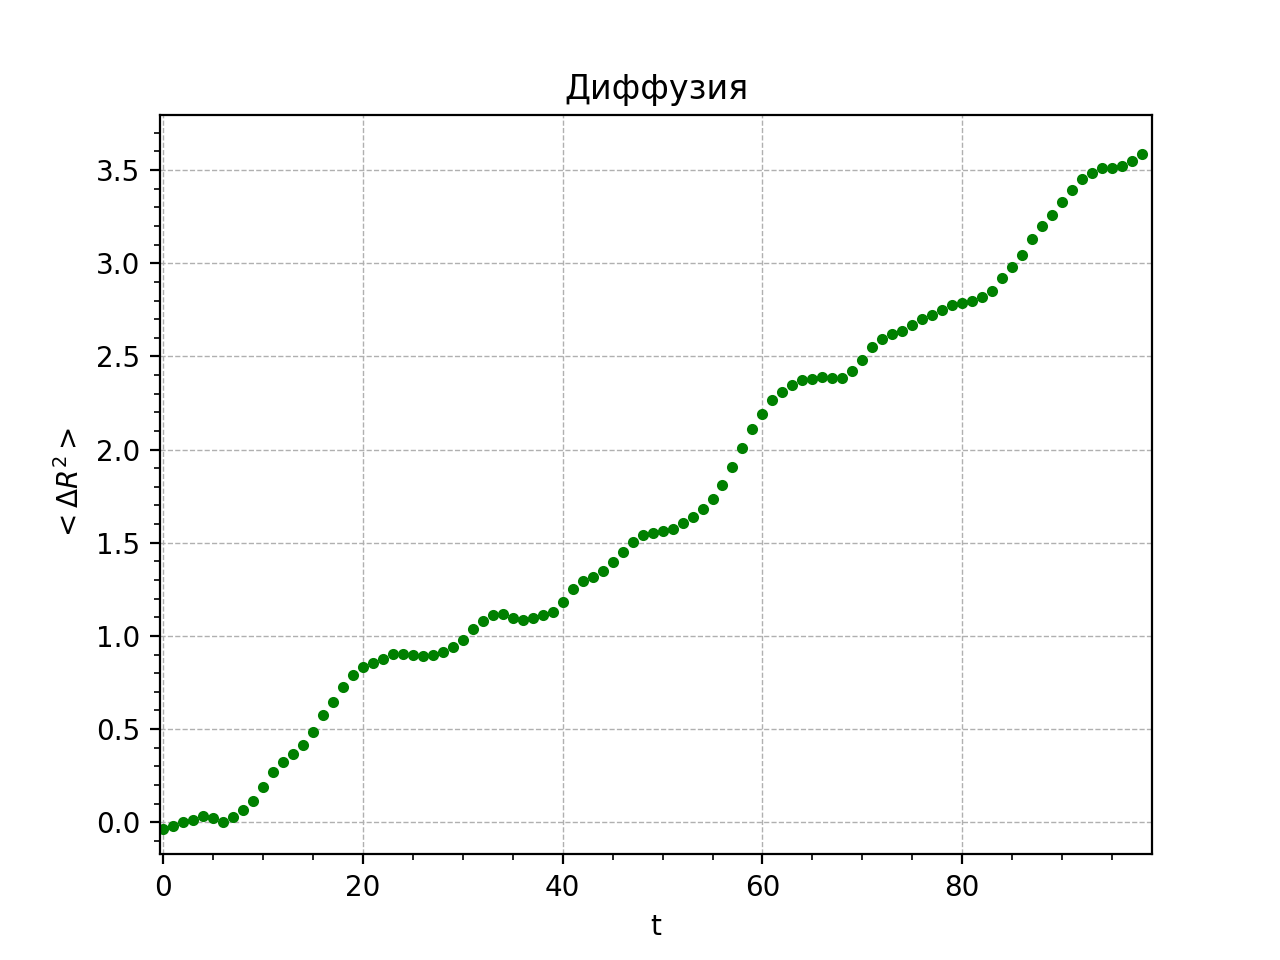
\includegraphics[width=\linewidth]{11.png}\\
        T = 1.0
    \end{center}
   
\end{minipage}
\begin{minipage}{0.47\textwidth}
    \begin{center}
        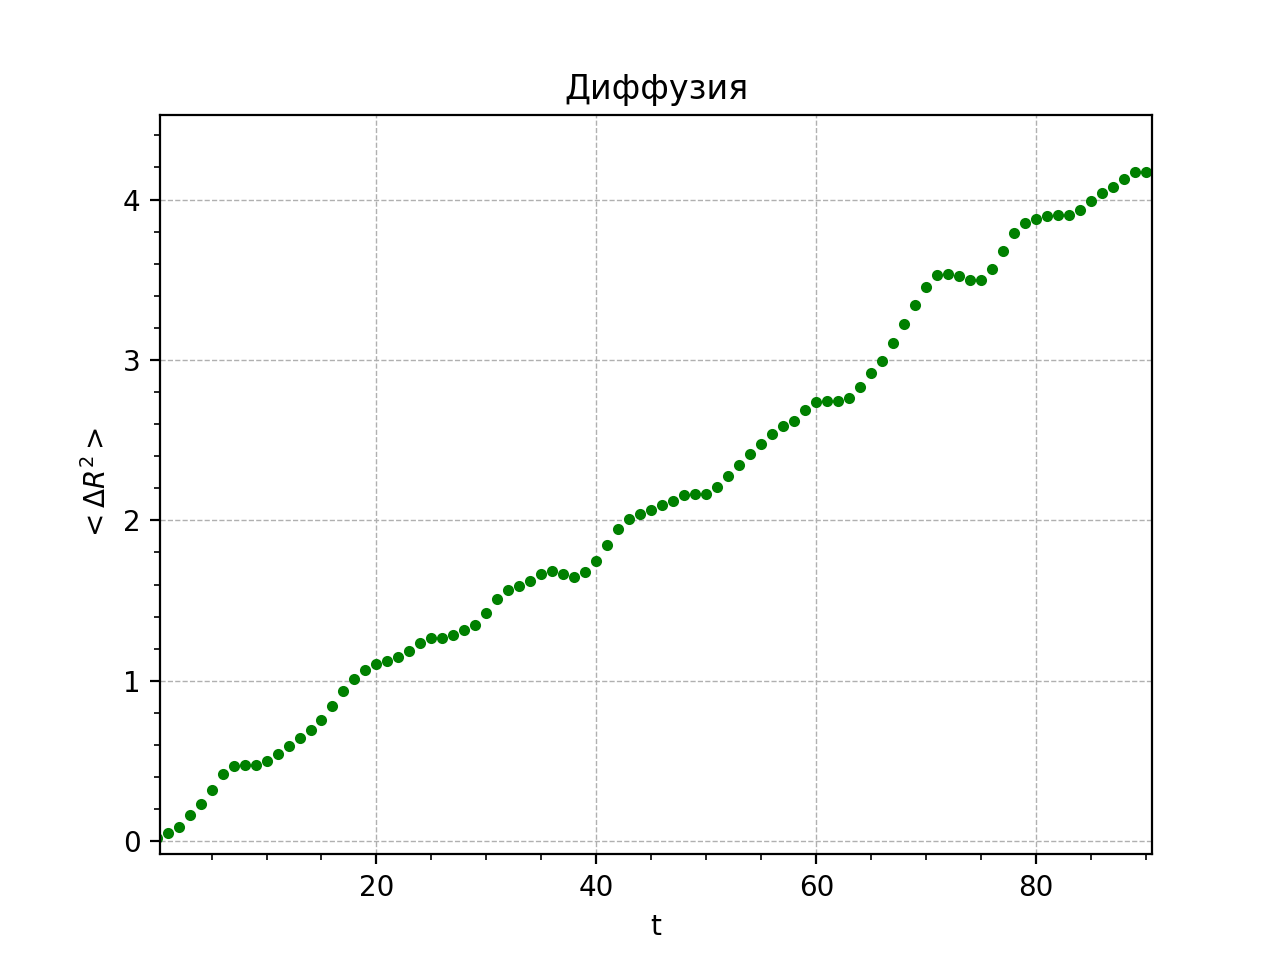
\includegraphics[width=\linewidth]{12.png}\\
        T = 2.0
    \end{center}
\end{minipage}

\section{$\log_{10}D = 0.05 + 0.07 \cdot P - \frac{1.04 + 0.1\cdot P}{  T}$}

Проверим формулу $\log_{10}D = 0.05 + 0.07 \cdot P - \frac{1.04 + 0.1\cdot P}{ T}$. Для удобстава, обозначим величину справа от знака равно за $f(T,P)$. 

\begin{center}
\begin{tabular}{|c|c|c|c|c|c|c|}
\hline
T&\rho&P&D&$\log_{10}D$&$f(T,P)$ & \Delta\%\\
\hline
0.8&0.50&0.352	&0.143&-0.844&	-1.269&38.6\%\\
\hline
0.8&0.60&0.672	&0.122&-0.869&	-1.289&27.5\%\\
\hline
0.8&0.70&1.226	&0.087&-1.117&	-1.317&15.4\%\\
\hline
0.8&0.80&3.521	&0.048&-1.319&	-1.444&8.6\%\\
\hline
0.8&0.85&3.856	&0.035&-1.455&	-1.462&1.6\%\\
\hline
\end{tabular}
\end{center}

Формула частично верна, что неудивительно, ведь возможность того, чтобы равенство соблюдалось, достигается только при значениях D $\ll$ 0.1, иначе, по данной формуле, давление при температуре, равной 0.8, должно быть отрицательным, что нефизично. 

 \begin{center}
   

    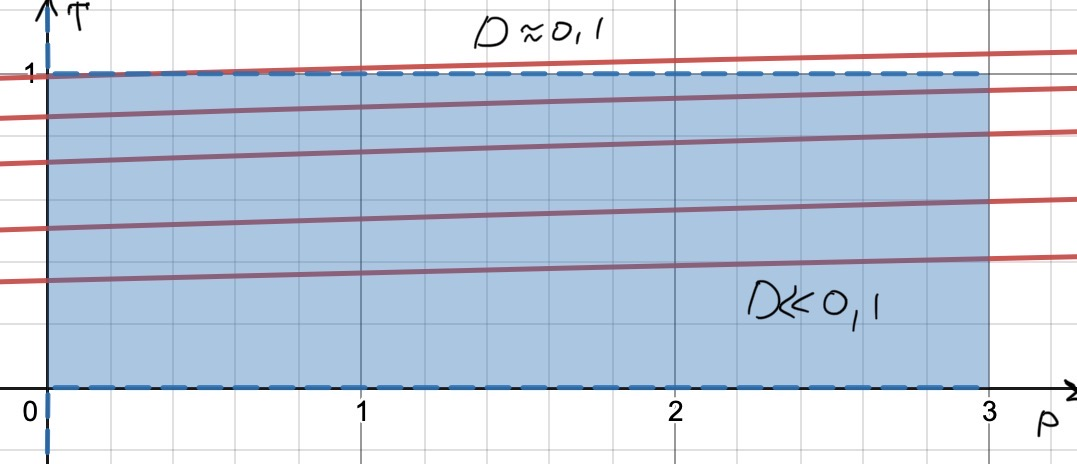
\includegraphics[width=0.8\linewidth]{t.JPG}\\
    Допустимые значения коэффициента D
    \end{center} 

\section{Заключение}

Код нужно переписать так, чтобы с ним было удобно работать и разбираться стороннему пользователю, однако все поставленные задачи выполнить удалось; полученные данные и зависимости схожи теоретическим, а так же полученным в других работах.
Github – https://github.com/Striz-lab/modelling/.
\end{document}
